\documentclass[spanish]{beamer}
\usepackage[utf8]{inputenc}
\usepackage{float}
\usepackage{beamerthemesplit}
\usepackage{latexsym}
\usepackage[T1]{fontenc}
\usepackage{amsmath}
\usepackage{hyperref}
\usepackage{graphicx}
\usepackage{babel,blindtext}
\usepackage{amsfonts}
\usepackage[round]{natbib}
\bibliographystyle{chicago}
\usepackage{subcaption} 


\decimalpoint

\usetheme{Antibes}%este es el templete que se usa a lo largo de la presentacion
%themes
%   default
%   Boadilla
%   Madrid
%   Pittsburgh
%   Copenhagen
%   Warsaw
%   Singapore
%   Malmoe
\newcommand\Fontvi{\fontsize{6}{7.2}\selectfont}
\mode<presentation>%tipo de 
\begin{document}

%%%%%%%%%%%%%%%%%%%%%%%%%%%%%%%%%%%%%%%%%%%%%%%%%%%%%%%%%%%%%%%%%%%%%%%%%%%%%%%%%%%%%%%%%%%%%%%%%%%%%%%%%%%%%
\title{Some Gambling Problems}
\author{Gamaliel Moreno Chávez}
\institute{MCPI}
\date{Ago-Dic\\ 2020}%para que ponga la fecha de hoy 

\frame{\titlepage}
%%%%%%%%%%%%%%%%%%%%%%%%%%%%%%%%%%%%%%%%%%%%%%%%%%%%%%%%%%%%%%%%%%%%%%%%%%%%%%%%%%%%%%%%%%%%%%%%%%%%%%%%%%%%%
%%%%%%%%%%%%%%%%%%%%%%%%%%%%%%%%%%%%%%%%%%%%%%%%%%%%%%%%%%%%%%%%%%%%%%%%%%%%%%%%%%%%%%%%%%%%%%%%%%%%%%%%%%%%%%%%%%%%%%%%%%%%%%%%%%%%%%%%%%%%%%%%%%%%%%%%%%%%%%%%%%%%%%%%%%%%%%%%%%%%%%%%%%%%%%%%%%%%%%%%%%%%%%%%%%%%%%%%%%
%%%%%%%%%%%%%%%%%%%%%%%%%%%%%%%%%%%%%%%%%%%%%%%%%%%%%%%%%%%%%%%%%%%%%%%%%%%%%%%%%%%%%%%%%%%%%%%%%%%%%%%%%%%%%%%%%%%%%%%%%%%%%%%%%%%%%%%%%%%%%%%%%%%%%%%%%%%%%%%%%%%%%%%%%%%%%%%%%%%%%%%%%%%%%%%%%%%%%%%%%%%%%%%%%%%%%%%%%%

\begin{frame}
\frametitle{Gambler’s ruin}
Consider a game of chance between two players: A, the gambler and B, the opponent. It is assumed that at each play, A either wins one unit from B with probability
$p$ or loses one unit to B with probability $q = 1 - p$. Conversely, B either wins from A or loses to A with probabilities q or p. The result of every play of the game is independent of the results of previous plays. The gambler A and the opponent B
each start with a given number of units and the game ends when either player has
lost his or her initial stake. What is the probability that the gambler loses all his or her money or wins all the opponent’s money, assuming that an unlimited number of
plays are possible?
\end{frame}

%%%%%%%%%%%%%%%%%%%%%%%%%%%%%%%%%%%%%%%%%%%%%%%%%%%%%%%%%%%%%%%%%%%%%%%%%%%%%%%%%%%%%%%%%%%%%%%%%%%%%%%%%%%%%
\begin{frame}
\frametitle{Gambler’s ruin}
This is the classic gambler’s ruin problem 1 . In a simple example
of gambler’s ruin, each play could depend on the spin of a fair coin, in which case
$p = q =1/2$ . The word ruin is used because if the gambler plays a fair game against a bank or casino with unlimited funds, then the gambler is certain to lose.
\end{frame}
%%%%%%%%%%%%%%%%%%%%%%%%%%%%%%%%%%%%%%%%%%%%%%%%%%%%%%%%%%%%%%%%%%%%%%%%%%%%%%%%%%%%%%%%%%%%%%%%%%%%%%%%%%%%%
\begin{frame}
\frametitle{Gambler’s ruin}
The result of each play of the game is a Bernoulli random variable which can only take the values -1 and +1. After a series of plays, we are interested in the current capital or stake of A, the gambler. This is simply the initial capital of A plus the sum of the values of the Bernoulli random variables generated by these plays. We are also interested in how the random variable which represents the current capital changes or evolves with the number of plays. This is measured at discrete points when the result of each play is known.

\end{frame}
%%%%%%%%%%%%%%%%%%%%%%%%%%%%%%%%%%%%%%%%%%%%%%%%%%%%%%%%%%%%%%%%%%%%%%%%%%%%%%%%%%%%%%%%%%%%%%%%%%%%%%%%%%%%%
\begin{frame}
\frametitle{Gambler’s ruin}
Suppose that $A$ has an initial capital of $k$ units and $B$ starts with $a - k$, where $a$ and $k$ are positive integers and $a > k$. If $X_n$ is a random variable representing A’s stake after $n$ plays (or at time point $n$), then initially $X_0 = k$. If $X_{n} = 0$, then the gambler A has lost (note that we must have $n \geq k$), whilst if $X_{n} = a (n  \geq a - k)$ then B is ruined, and in both cases the game terminates. Our initial objective is the derivation of $P(X_{n} = 0)$ for all $n \geq k$.
\end{frame}
%%%%%%%%%%%%%%%%%%%%%%%%%%%%%%%%%%%%%%%%%%%%%%%%%%%%%%%%%%%%%%%%%%%%%%%%%%%%%%%%%%%%%%%%%%%%%%%%%%%%%%%%%%%%%
\begin{frame}
\frametitle{Gambler’s ruin}
\begin{itemize}
\item The sequence of random variables $X_{0} , X_{1} , X_{2}$ is a random process.
\item Finite sample, from 0 to a. 
\item These values are known as the \textbf{state} of the process at each \textbf{stage} or time point n
\end{itemize}
\end{frame}
%%%%%%%%%%%%%%%%%%%%%%%%%%%%%%%%%%%%%%%%%%%%%%%%%%%%%%%%%%%%%%%%%%%%%%%%%%%%%%%%%%%%%%%%%%%%%%%%%%%%%%%%%%%%%
\begin{frame}
\frametitle{Gambler’s ruin}
If $C_{k}$ is the event that $A$ is eventually ruined
\begin{equation*}
P(C_{k})= \displaystyle \sum_{n=k}^{\infty}P(X_{n}=0)
\end{equation*}
Note also that the results of each trial are independent, but $X_{n} , n = 0, 1, 2,\ldots$  are not.

\end{frame}
%%%%%%%%%%%%%%%%%%%%%%%%%%%%%%%%%%%%%%%%%%%%%%%%%%%%%%%%%%%%%%%%%%%%%%%%%%%%%%%%%%%%%%%%%%%%%%%%%%%%%%%%%%%%%
\begin{frame}
\frametitle{Gambler’s ruin}
This is easily seen to be true by considering a particular value of $X _{n}$, say $x$, $(0 < x < a)$, after $n$ plays, say. This event may only occur if previously $X_{n-1} = x - 1$  or $x + 1$.

The state reached in any play depends on the state of the previous play only: in other words the process is said to display the \textbf{Markov} property, of which more will be explained later.
\end{frame}
%%%%%%%%%%%%%%%%%%%%%%%%%%%%%%%%%%%%%%%%%%%%%%%%%%%%%%%%%%%%%%%%%%%%%%%%%%%%%%%%%%%%%%%%%%%%%%%%%%%%%%%%%%%%%
\begin{frame}
\frametitle{Gambler’s ruin}
Clearly the calculation of $P(X n = 0)$ for all $n$ is likely to be a long and tedious
process. We now introduce the solution of \textbf{linear homogeneous difference equations.}
\end{frame}
%%%%%%%%%%%%%%%%%%%%%%%%%%%%%%%%%%%%%%%%%%%%%%%%%%%%%%%%%%%%%%%%%%%%%%%%%%%%%%%%%%%%%%%%%%%%%%%%%%%%%%%%%%%%%
\begin{frame}
\frametitle{Gambler’s ruin}
if we define $u_k = P(C_k)$, then after the first play the probability of ruin is either $u{k+1} = P(C_{k+1} )$ or $u_{k-1} = P(C_{k-1})$. Let us consider the result of the first play,and define $D$ to be the event that $A$ wins, and the complement $D^{c}$ the event that $A$ loses. Using the law of total probability it follows that

\begin{equation*}
P(C_{k}) = P(C_{k}|D)P(D) + P(C_k \vert D^{c} )P(D^{c}).
\end{equation*}
\end{frame}

%%%%%%%%%%%%%%%%%%%%%%%%%%%%%%%%%%%%%%%%%%%%%%%%%%%%%%%%%%%%%%%%%%%%%%%%%%%%%%%%%%%%%%%%%%%%%%%%%%%%%%%%%%%%%
\begin{frame}
\frametitle{Gambler’s ruin}
As remarked previously, event $C_{k}$ given a win, namely $C_{k} \vert D$ becomes event $C_{k+1}$. Hence $P(C_{k} \vert D) = P(C_{k+1} )$. Similarly $P(C_{k} \vert D^{c} ) = P(C_{k-1} )$. Also $P(D) = p$ and $P(D_{c}) = q$, which means that Eqn can be written as

\begin{equation*}
u_{k} = u_{k+1} p + u_{k-1} q, \quad (1 \leq k \leq a -1).
\end{equation*}
This equation can be re-arranged into

\begin{equation*}
 p u_{k+1} -u_{k}+ qu_{k-1} = 0
\end{equation*}
which is a second-order linear homogeneous difference equation

\end{frame}

%%%%%%%%%%%%%%%%%%%%%%%%%%%%%%%%%%%%%%%%%%%%%%%%%%%%%%%%%%%%%%%%%%%%%%%%%%%%%%%%%%%%%%%%%%%%%%%%%%%%%%%%%%%%%
\begin{frame}
\frametitle{Gambler’s ruin}
If the gambler starts with zero stake, then ruin is certain, whilst if the gambler starts with all the capital a, then ruin is impossible. These translate into
\begin{equation*}
u_{0} = P(C_{0}) = 1 \quad \text{and} \quad u_{a} = P(C_{a}) = 0,
\end{equation*}
which are the \textbf{boundary conditions} for the difference equation
\end{frame}
%%%%%%%%%%%%%%%%%%%%%%%%%%%%%%%%%%%%%%%%%%%%%%%%%%%%%%%%%%%%%%%%%%%%%%%%%%%%%%%%%%%%%%%%%%%%%%%%%%%%%%%%%%%%%
\begin{frame}
\frametitle{Gambler’s ruin}
Solving the differential equation
\begin{block}{Probability of ruin}
\begin{equation*}
u_{k}=\frac{s^k-s^a}{1-s^a}, \quad (p\neq \frac{1}{2} )
\end{equation*}

\begin{equation*}
u_{k}=\frac{a-k}{a}, \quad (p= \frac{1}{2} )
\end{equation*}
\end{block}


\end{frame}

%%%%%%%%%%%%%%%%%%%%%%%%%%%%%%%%%%%%%%%%%%%%%%%%%%%%%%%%%%%%%%%%%%%%%%%%%%%%%%%%%%%%%%%%%%%%%%%%%%%%%%%%%%%%%
\begin{frame}
\frametitle{Probability of ruin}
Numerical simulations
\begin{center}
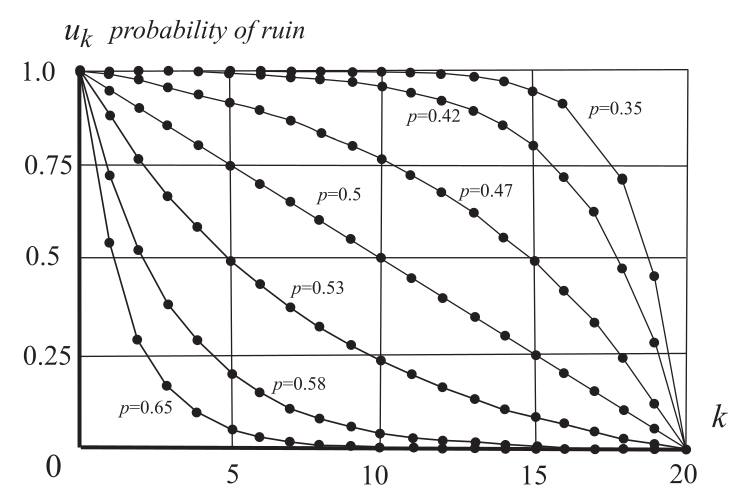
\includegraphics[scale=0.35]{im1.png}
\end{center}

\end{frame}



%%%%%%%%%%%%%%%%%%%%%%%%%%%%%%%%%%%%%%%%%%%%%%%%%%%%%%%%%%%%%%%%%%%%%%%%%%%%%%%%%%%%%%%%%%%%%%%%%%%%%%%%%%%%%
\begin{frame}
\frametitle{Duration of the game}
It is natural in the gambler’s ruin problem to be curious about how long, or really
how many plays we would expect the game to last.\vspace{1em}


Two variables: $k$, the initial capital, and $n$, the remaining number of plays until the end of the game.Now $n$ is unknown, and is a value of the random variable $N$ which depends, in turn, on the results of the remaining plays.\vspace{1em}


Let $p(n\vert k)$ be the conditional probability that the game ends in $n$ steps given that the initial capital is $k$. the $n$ will be any positive integer greater than or equal to the smaller of $k$ and $a - k$.
\end{frame}
%%%%%%%%%%%%%%%%%%%%%%%%%%%%%%%%%%%%%%%%%%%%%%%%%%%%%%%%%%%%%%%%%%%%%%%%%%%%%%%%%%%%%%%%%%%%%%%%%%%%%%%%%%%%%
\begin{frame}
\frametitle{Duration of the game}
\begin{block}{Expected duration}
Let the random variable $N$ be the number of plays until the game ends, and let $K$ be the random variable of the initial stake. The expected number of plays to termination will be 
\begin{equation*}
E(N\vert K)= \sum_{n=0}^{\infty}{np(n\vert k)}=d_{k}
\end{equation*}
\end{block}
$p(n\vert k)$ is a probability function and must therefore satisfy

\begin{equation*}
\sum_{n=0}^{\infty}{p(n\vert k)}=1
\end{equation*}
\end{frame}
%%%%%%%%%%%%%%%%%%%%%%%%%%%%%%%%%%%%%%%%%%%%%%%%%%%%%%%%%%%%%%%%%%%%%%%%%%%%%%%%%%%%%%%%%%%%%%%%%%%%%%%%%%%%%
\begin{frame}
\frametitle{Duration of the game}

After the result of the next play is known, then the process will move from step $(k, n)$ to either step $(k + 1, n - 1)$ with probability p, or to step $(k - 1, n - 1)$ with probability $q = 1-p$. By the law of total probability, it follows
that

\begin{equation*}
p(n\vert k) = p(n -1\vert k + 1)p + p(n -1\vert k -1)q
\end{equation*}

Substituting for $p(n\vert k)$ in $d_{k}= \sum_{n=0}^{\infty}{np(n\vert k)}$
\begin{equation*}
d_{k} = p \sum_{n=1}^{\infty} np(n-1 \vert k+1)+ q \sum_{n=1}^{\infty}np(n -1\vert k -1)
\end{equation*}

The change of variable $r = n - 1$ leads to

\begin{equation*}
d_{k} = p \sum_{r=0}^{\infty} (r+1)p(r \vert k+1)+ q \sum_{r=0}^{\infty}(r+1)p(r\vert k -1)
\end{equation*}
\end{frame}
%%%%%%%%%%%%%%%%%%%%%%%%%%%%%%%%%%%%%%%%%%%%%%%%%%%%%%%%%%%%%%%%%%%%%%%%%%%%%%%%%%%%%%%%%%%%%%%%%%%%%%%%%%%%%
\begin{frame}
\frametitle{Duration of the game}

\begin{equation*}
d_{k} = p \sum_{r=0}^{\infty} (r+1)p(r \vert k+1)+ q \sum_{r=0}^{\infty}(r+1)p(r\vert k -1)
\end{equation*}
reorder 

\begin{multline*}
d_{k} = p \sum_{r=1}^{\infty} (r)p(r \vert k+1)+ q \sum_{r=1}^{\infty}(r)p(r\vert k -1)+ \\
p \sum_{r=0}^{\infty} p(r \vert k+1)+ q \sum_{r=0}^{\infty}p(r\vert k -1)
\end{multline*}

 
\begin{equation*}
d_{k} = p \sum_{r=1}^{\infty} (r)p(r \vert k+1)+ q \sum_{r=1}^{\infty}(r)p(r\vert k -1)+p+q
\end{equation*}
\end{frame}
%%%%%%%%%%%%%%%%%%%%%%%%%%%%%%%%%%%%%%%%%%%%%%%%%%%%%%%%%%%%%%%%%%%%%%%%%%%%%%%%%%%%%%%%%%%%%%%%%%%%%%%%%%%%%
\begin{frame}
\frametitle{Duration of the game}
Hence the expected duration $d_{k}$ satisfies the difference equation

\begin{equation*}
d_{k} = p d_{k+1} + q d_{k-1} + 1, \quad (k \geq 1)
\end{equation*}

where
\begin{equation*}
d_{k+1} = p \sum_{r=1}^{\infty} (r)p(r \vert k+1) \quad \text{  and  } \quad d_{k-1}=\sum_{r=1}^{\infty}(r)p(r\vert k -1)
\end{equation*}
This is a linear inhomogeneous second-order difference equation. The boundary conditions are obtained by $k = 0$ and $k = a$, then the game terminates so that the expected durations must be zero, that is, 
\begin{equation*}
d_{0} = d_{a} = 0.
\end{equation*}


\end{frame}

%%%%%%%%%%%%%%%%%%%%%%%%%%%%%%%%%%%%%%%%%%%%%%%%%%%%%%%%%%%%%%%%%%%%%%%%%%%%%%%%%%%%%%%%%%%%%%%%%%%%%%%%%%%%%
\begin{frame}
\frametitle{Duration of the game}
\begin{block}{expected duration}
\begin{equation*}
d_{k} = k(a - k), \quad p = q
\end{equation*}
\begin{equation*}
d_{k} = \frac{1}{1-2p} \left[  k-\frac{a(1-s^k)}{1-s^a} \right] , \quad q \neq q
\end{equation*}


\end{block}

\end{frame}


%%%%%%%%%%%%%%%%%%%%%%%%%%%%%%%%%%%%%%%%%%%%%%%%%%%%%%%%%%%%%%%%%%%%%%%%%%%%%%%%%%%%%%%%%%%%%%%%%%%%%%%%%%%%%
\begin{frame}
\frametitle{Duration of the game}
Numerical simulations
\begin{center}
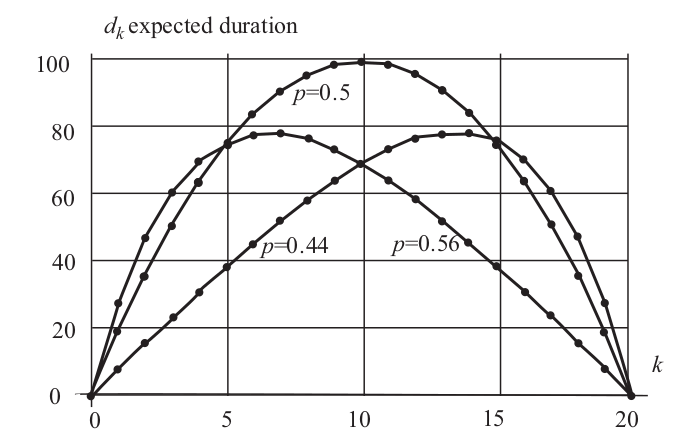
\includegraphics[scale=0.4]{im2.png}
\end{center}

\end{frame}



%%%%%%%%%%%%%%%%%%%%%%%%%%%%%%%%%%%%%%%%%%%%%%%%%%%%%%%%%%%%%%%%%%%%%%%%%%%%%%%%%%%%%%%%%%%%%%%%%%%%%%%%%%%%%
\end {document}



                                                  






